\documentclass{beamer}

\newcommand{\lesson}{{\tt Stacks and Queues}}


\newcommand{\course}{Introduction to Object-Oriented Programming}
\subject{\course}
\title[\lesson]{\course}
\subtitle{\lesson}

\author[CS 1331]
{Christopher Simpkins \\\texttt{chris.simpkins@gatech.edu}}
\institute[Georgia Tech]

\date[]{}

\newcommand{\link}[2]{\href{#1}{\textcolor{blue}{\underline{#2}}}}
\newcommand{\code}{http://www.cs1331.org/code}

\usepackage{colortbl}

% If you have a file called "university-logo-filename.xxx", where xxx
% is a graphic format that can be processed by latex or pdflatex,
% resp., then you can add a logo as follows:

% \pgfdeclareimage[width=0.6in]{coc-logo}{cc_2012_logo}
% \logo{\pgfuseimage{coc-logo}}

\mode<presentation>
{
  \usetheme{Berlin}
  \useoutertheme{infolines}

  % or ...

 \setbeamercovered{transparent}
  % or whatever (possibly just delete it)
}

\usepackage{tikz}
% Optional PGF libraries
\usepackage{pgflibraryarrows}
\usepackage{pgflibrarysnakes}
\usepackage{pgfplots}
\usepackage{fancybox}
\usepackage{listings}
\usepackage{hyperref}
\hypersetup{colorlinks=true,urlcolor=blue}
\usepackage[english]{babel}
% or whatever

\usepackage[latin1]{inputenc}
% or whatever

\usepackage{times}
\usepackage[T1]{fontenc}
% Or whatever. Note that the encoding and the font should match. If T1
% does not look nice, try deleting the line with the fontenc.


\usepackage{listings}

% "define" Scala
\lstdefinelanguage{scala}{
  morekeywords={abstract,case,catch,class,def,%
    do,else,extends,false,final,finally,%
    for,if,implicit,import,match,mixin,%
    new,null,object,override,package,%
    private,protected,requires,return,sealed,%
    super,this,throw,trait,true,try,%
    type,val,var,while,with,yield},
  otherkeywords={=>,<-,<\%,<:,>:,\#,@},
  sensitive=true,
  morecomment=[l]{//},
  morecomment=[n]{/*}{*/},
  morestring=[b]",
  morestring=[b]',
  morestring=[b]""",
}

\usepackage{color}
\definecolor{dkgreen}{rgb}{0,0.6,0}
\definecolor{gray}{rgb}{0.5,0.5,0.5}
\definecolor{mauve}{rgb}{0.58,0,0.82}

% Default settings for code listings
\lstset{frame=tb,
  language=scala,
  aboveskip=2mm,
  belowskip=2mm,
  showstringspaces=false,
  columns=flexible,
  basicstyle={\scriptsize\ttfamily},
  numbers=none,
  numberstyle=\tiny\color{gray},
  keywordstyle=\color{blue},
  commentstyle=\color{dkgreen},
  stringstyle=\color{mauve},
  frame=single,
  breaklines=true,
  breakatwhitespace=true,
  keepspaces=true
  %tabsize=3
}


% If you wish to uncover everything in a step-wise fashion, uncomment
% the following command:

\beamerdefaultoverlayspecification{<+->}


\begin{document}

\begin{frame}
  \titlepage
\end{frame}

%------------------------------------------------------------------------
\begin{frame}[fragile]{Stacks and Queues}

\begin{itemize}
\item Stacks
\item Queues
\item Design Exercise
\end{itemize}


\end{frame}
%------------------------------------------------------------------------

%------------------------------------------------------------------------
\begin{frame}[fragile]{What is a stack?}


\begin{center}

\includegraphics[height=2.25in]{episode-3-mike-jesse-walt.jpg}\footnote{Source:\url{http://blogs.amctv.com/breaking-bad/photo-galleries/breaking-bad-season-5-episode-photos/}}\\
Fat stacks
\end{center}

\end{frame}
%------------------------------------------------------------------------

%------------------------------------------------------------------------
\begin{frame}[fragile]{What is a stack?}


\begin{center}
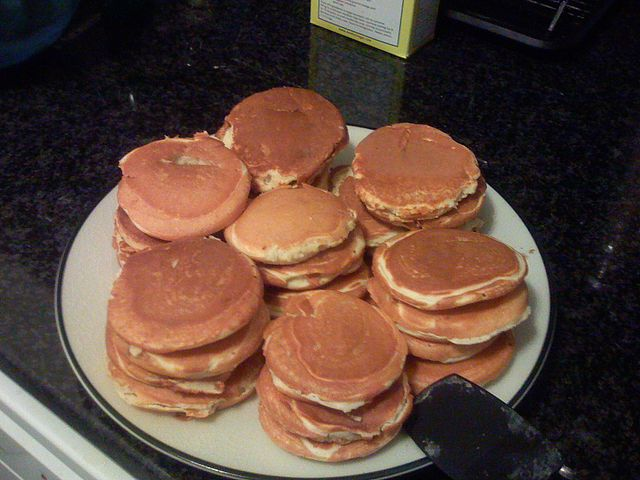
\includegraphics[height=2.25in]{640px-Silver_dollar_pancakes.jpeg}\footnote{Source:"Silver dollar pancakes" by Ehedaya at en.wikipedia - Own work (Original caption: "self-made"). Licensed under Public domain via Wikimedia Commons - \url{http://commons.wikimedia.org/wiki/File:Silver_dollar_pancakes.JPG\#mediaviewer/File:Silver_dollar_pancakes.JPG}}\\
Tasty stacks
\end{center}

\end{frame}
%------------------------------------------------------------------------

%------------------------------------------------------------------------
\begin{frame}[fragile]{Gratuitous Super Troopers}


\begin{center}
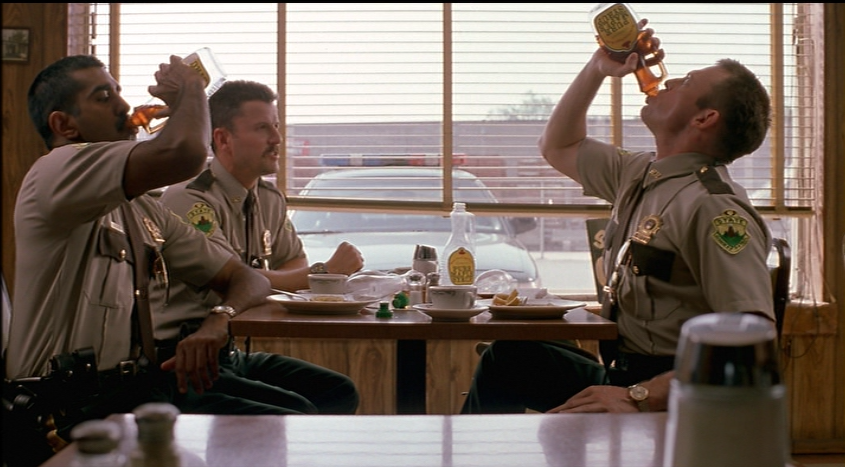
\includegraphics[height=2.25in]{syrup.png}\footnote{Source: \url{http://sumidiot.blogspot.com/2010/05/super-troopers.html}}
\end{center}

\end{frame}
%------------------------------------------------------------------------


%------------------------------------------------------------------------
\begin{frame}[fragile]{Stack ADT}

Data:
\begin{itemize}
  \item a list of elements
\end{itemize}

A {\it stack} is a LIFO (last in, first out) data structure with two defining operations:
\begin{itemize}
\item {\it push} adds an element to the stack
\item {\it pop} returns and removes the most recently added element from the stack
\end{itemize}

A stack may also have
\begin{itemize}
\item an {\it isEmpty} operation, which is good style but not strictly necessary.
\item a {\it peek} operation, which returns the next element to be removed from the stack with a pop operation but does not remove it.
\end{itemize}



\end{frame}
%------------------------------------------------------------------------

%------------------------------------------------------------------------
\begin{frame}[fragile]{ArrayList Stack Implementation}

\vspace{-.05in}
A stack can be implemented easily using {\tt ArrayList}

\begin{itemize}
\item {\it push} adds elements to the end of the {\tt ArrayList}.
\item {\it pop} removes and returns the last element in the {\tt ArrayList}.
\item {\it isEmpty} delegates to {\tt ArrayList}'s {\tt isEmpty} method.
\end{itemize}

The entire implementation (as an inner class) is:
\begin{lstlisting}[language=Java]
    static class Stack<E> {
        private ArrayList<E> elems = new ArrayList<>();

        public void push(E item) {
            elems.add(item);
        }
        public E pop() {
            return elems.remove(elems.size() - 1);
        }
        public boolean isEmpty() {
            return elems.isEmpty();
        }
    }
\end{lstlisting}
\vspace{-.05in}
See \link{\code/data-structures/ArrayListDataStructures.java}{ArrayListDataStructures.java}.

\end{frame}
%------------------------------------------------------------------------

%------------------------------------------------------------------------
\begin{frame}[fragile]{Linked Stack Implementation}


Here's a stack implemented with {\tt Node}s.
\begin{lstlisting}[language=Java]
public class LinkedStack<E> {
    private class Node<E> {
        E data;
        Node<E> next;

        Node(E data, Node<E> next) { this.data=data; this.next=next; }
    }
    private Node<E> head;

    public void push(E item) {
        head = new Node<E>(item, head);
    }
    public E pop() {
        E answer = head.data;
        head = head.next;
        return answer;
    }
    public boolean isEmpty() { return (head == null); }
}
\end{lstlisting}
\vspace{-.05in}
Look familiar? See \link{\code/data-structures/LinkedStack.java}{LinkedStack.java}.

\end{frame}
%------------------------------------------------------------------------

%------------------------------------------------------------------------
\begin{frame}[fragile]{Queue ADT}

Data:
\begin{itemize}
  \item a list of elements
\end{itemize}

A {\it queue} is a FIFO (first in, first out) data structure with two defining operations:
\begin{itemize}
\item {\it enqueue} adds an element to the queue
\item {\it dequeue} returns and removes the least recently added element from the queue
\end{itemize}

A queue may also have
\begin{itemize}
\item an {\it isEmpty} operation, which is good style but not strictly necessary.
\item a {\it peek} operation, which returns the next element to be removed from the queue with a dequeue operation but does not remove it.
\end{itemize}

\end{frame}
%------------------------------------------------------------------------

%------------------------------------------------------------------------
\begin{frame}[fragile]{ArrayList Queue Implementation}

\vspace{-.05in}
A queue can be implemented easily using {\tt ArrayList}

\begin{itemize}
\item {\it enqueue} adds elements to the end of the {\tt ArrayList}.
\item {\it dequeue} removes and returns the first element in the {\tt ArrayList}.
\item {\it isEmpty} delegates to {\tt ArrayList}'s {\tt isEmpty} method.
\end{itemize}

The entire implementation (as an inner class) is:
\begin{lstlisting}[language=Java]
    static class Queue<E> {
        private ArrayList<E> elems = new ArrayList<>();

        public void enqueue(E item) {
            elems.add(item);
        }
        public E dequeue() {
            return elems.remove(0);
        }
        public boolean isEmpty() {
            return elems.isEmpty();
        }
    }
\end{lstlisting}
\vspace{-.05in}
See \link{\code/data-structures/ArrayListDataStructures.java}{ArrayListDataStructures.java}.

\end{frame}
%------------------------------------------------------------------------

%------------------------------------------------------------------------
\begin{frame}[fragile]{Linked Queue Implementation}

\vspace{-.05in}
\begin{lstlisting}[language=Java]
public class LinkedQueue<E> {
    private class Node<E> ...
    private Node<E> head;
    private Node<E> last;

    public void enqueue(E item) {
        Node<E> newNode = new Node<E>(item, null);
        if (null == head) head = newNode;
        if (null != last) last.next = newNode;
        last = newNode;
    }
    public E dequeue() {
        E answer = head.data;
        head = head.next;
        return answer;
    }
    public boolean isEmpty() { return (head == null); }
}
\end{lstlisting}
\vspace{-.05in}
Essentially same as {\tt LinkedStack}, except we maintain a {\tt last} reference and add elements to the end intead of the head.  See \link{\code/data-structures/LinkedQueue.java}{LinkedQueue.java}.

\end{frame}
%------------------------------------------------------------------------

%------------------------------------------------------------------------
\begin{frame}[fragile]{Comparing ArrayList and Linked Implementations}


Here, again, is the {\tt dequeue} method in {\tt ArrayListQueue}:
\begin{lstlisting}[language=Java]
  private ArrayList<E> elems = new ArrayList<>();
  public E dequeue() {
      return elems.remove(0);
  }
\end{lstlisting}

And here is the {\tt dequeue} method in {\tt LinkedQueue}:
\begin{lstlisting}[language=Java]
  public E dequeue() {
      E answer = head.data;
      head = head.next;
      return answer;
    }
\end{lstlisting}

\begin{itemize}
\item<1-> What is the Big-O of the {\tt dequeue} method in {\tt ArrayListQueue}?
\begin{itemize}
\item<2-> $\mathcal{O}(n)$.
\end{itemize}
\item<3-> What is the Big-O of the {\tt dequeue} method in {\tt LinkedQueue}?
\begin{itemize}
\item<4-> $\mathcal{O}(1)$.
\end{itemize}
\end{itemize}

\end{frame}
%------------------------------------------------------------------------

%------------------------------------------------------------------------
\begin{frame}[fragile]{Design Exercise}


Our data structures implement the core elements of their ADTs, but there are some problems from an OO design standpoint.
\begin{itemize}
\item What happens if you call {\tt pop} on an empty {\tt ArrayListStack}?
\item What happens if you call {\tt pop} on an empty {\tt LinkedStack}?
\item What if you start off using an {\tt ArrayListStack} but then decide to switch to using a {\tt LinkedStack}?
\end{itemize}


\end{frame}
%------------------------------------------------------------------------

%------------------------------------------------------------------------
\begin{frame}[fragile]{Designing Error Reports}


Calling {\tt pop} on an empty {\tt ArrayListStack} results in:
\begin{lstlisting}[language=Java]
Exception in thread "main" java.lang.ArrayIndexOutOfBoundsException: -1
\end{lstlisting}

Calling {\tt pop} on an empty {\tt LinkedStack} results in:
\begin{lstlisting}[language=Java]
Exception in thread "main" java.lang.NullPointerException
\end{lstlisting}
There are two problems with these error reports:
\begin{itemize}
\item They leak implementation details across an abstraction boundary - why should a user know that a stack is implemented using arrays?
\item They don't report the actual user error that caused the exception - calling {\tt pop} on an empty stack.
\end{itemize}

We can fix these design problems by throwing {\tt java.util.EmptyStackException} in the {\tt pop} methods if the stack is empty.

\end{frame}
%------------------------------------------------------------------------

%------------------------------------------------------------------------
\begin{frame}[fragile]{A Stack Interface}

We could have both of our implementations implement a {\tt Stack} interface:
\begin{lstlisting}[language=Java]
public interface Stack<E> {

    public void push(E item);

    public E pop() throws java.util.EmptyStackException;

    public abstract boolean isEmpty();
}
\end{lstlisting}
Is there a problem with this approach?
\begin{itemize}
\item<2> {\tt java.util.EmptyStackException} is-a {\tt RuntimExecption}, which is not checked, so implementing classes will not be required to declare it.
\end{itemize}


\end{frame}
%------------------------------------------------------------------------

%------------------------------------------------------------------------
\begin{frame}[fragile]{{\tt AbstractStack}}


Abstract classes to the rescue!
\begin{lstlisting}[language=Java]
public abstract class AbstractStack<E> implements Stack<E> {
    public final E pop() {
        if (isEmpty()) { throw new java.util.EmptyStackException(); }
        return removeNext();
    }
    protected abstract E removeNext();
}
\end{lstlisting}

\begin{itemize}
\item This {\tt pop} method will be the one and only pop method used by subclasses (because it's final), ensuring that {\tt java.util.EmptyStackException} is thrown as we want.
\item Subclasses must implement {\tt removeNext()}, which does what their {\tt pop} methods used to do and is not visible to clients because it's {\tt protected}.
\end{itemize}

So all we have to do is extend {\tt AbstractStack} and change the name of our {\tt pop} methods to {\tt removeNext}.

\end{frame}
%------------------------------------------------------------------------

%------------------------------------------------------------------------
\begin{frame}[fragile]{Closing Thoughts}


Today we
\begin{itemize}
\item learned about two basic data structures: stacks and queues,
\item learned about alternative data structure implementations,
\item applied exception programming principles,
\item designed an OO family of stack classes, and
\item used Java langauge features (like abstract classes and methods, final methods, and protected methods) to implement our OO stack family design.
\end{itemize}


\end{frame}
%------------------------------------------------------------------------

%------------------------------------------------------------------------
\begin{frame}[fragile]{Programming Exercise}

A string is said to have balanced parentheses if for every open paren there is a matching close paren that comes after it, and no closing paren occurs before a corresponding open paren.  This is an example of a string with balanced parentheses:
\begin{lstlisting}[language=Java]
(map (lambda (x) (* x x)) (list 1 2 3 4))
\end{lstlisting}
and this is an example of unbalanced parentheses:
\begin{lstlisting}[language=Java]
(map (lambda (x) (* x x)) (list 1 2 3 4)))
\end{lstlisting}
\vspace{-.05in}
\begin{itemize}
\item Write a method {\tt public static boolean hasBalancedParens(String s)} that returns {\tt true} if {\tt s} contains balanced parentheses, {\tt false} otherwise.
\item Write a method {\tt public static boolean isBalanced(String s)} that checks for balanced ``parentheses'' of many types, for example, {\tt ( [ ] ) \{ \}} is balanced, but {\tt  [ \{ ] \}} is not.
\end{itemize}


\end{frame}
%------------------------------------------------------------------------


% %------------------------------------------------------------------------
% \begin{frame}[fragile]{}


% \begin{lstlisting}[language=Java]

% \end{lstlisting}

% \begin{itemize}
% \item
% \end{itemize}


% \end{frame}
% %------------------------------------------------------------------------


\end{document}
